
\documentclass[handout]{beamer}
\usepackage{framed}
\usepackage{geometry}
\usetheme{metropolis}
\usepackage{tikz}
\usetikzlibrary{shadows}
\geometry{paperwidth=14.25cm,paperheight=10cm}
\setbeamertemplate{navigation symbols}{}
\setbeamertemplate{frametitle}[default][center]
\setbeamersize{text margin left=15pt,text margin right=15pt}
\usefonttheme{serif}
\setbeamerfont{frametitle}{size=\Huge}
\definecolor{codegreen}{rgb}{0,0.6,0}
\definecolor{codered}{rgb}{0.6,0,0}
\newenvironment{greenframe}{%
	\setbeamercolor{frametitle}{bg=codegreen}
	\begin{frame}
	}{%
	\end{frame}
}
\setbeamercolor{frametitle}{bg=codered}
\usepackage{graphicx}
\usepackage[most]{tcolorbox}
\setbeamertemplate{navigation symbols}{}
\setbeamertemplate{frametitle}{%
	\nointerlineskip%
	\begin{beamercolorbox}[wd=\paperwidth,ht=3.5ex,dp=2ex]{frametitle}
		\centering
		\hspace*{1ex}\insertframetitle%
	\end{beamercolorbox}%
}
\begin{document}

\begin{frame}[plain]{Reviewer 2}
    \begin{columns}
        \begin{column}{0.5\textwidth}
            \centering
            \tikz\node[inner sep=0pt, draw=none, drop shadow={shadow xshift=1mm,shadow yshift=-1mm,fill=black, opacity=0.3}]{
                
\includegraphics[width=\linewidth]{images/br_role_1}
            };
        \end{column}
        \begin{column}{0.5\textwidth}
            \begin{tcolorbox}[colback=white,colframe=codered,fonttitle=\bfseries, title=Reviewer 2]
                Reviewer 2 is an academic legend who's never met a paper he liked. His feedback always begins with `I enjoyed reading this, however...' followed by countless critiques. If you are lucky, you get a `Weak Reject'. Rumor has it, if your rejection didn't make you cry, you didn't get Reviewer 2.
            \end{tcolorbox}
        \end{column}
    \end{columns}
\end{frame}

\begin{frame}[plain]{Rejecting Reviewer}
    \begin{columns}
        \begin{column}{0.5\textwidth}
            \centering
            \tikz\node[inner sep=0pt, draw=none, drop shadow={shadow xshift=1mm,shadow yshift=-1mm,fill=black, opacity=0.3}]{
                
\includegraphics[width=\linewidth]{images/br_role_2}
            };
        \end{column}
        \begin{column}{0.5\textwidth}
            \begin{tcolorbox}[colback=white,colframe=codered,fonttitle=\bfseries, title=Doktor Schon Gehört]
                Doktor Schon Gehört always has a nostalgic air about him, endlessly droning on about old academic papers nobody else recalls. Like a broken record, he can't resist pointing out, `Schon gehört!' (Already heard), as if the world of research began and ended with his reading list.
            \end{tcolorbox}
        \end{column}
    \end{columns}
\end{frame}

\begin{frame}[plain]{Rejecting Reviewer}
    \begin{columns}
        \begin{column}{0.5\textwidth}
            \centering
            \tikz\node[inner sep=0pt, draw=none, drop shadow={shadow xshift=1mm,shadow yshift=-1mm,fill=black, opacity=0.3}]{
                
\includegraphics[width=\linewidth]{images/br_role_3}
            };
        \end{column}
        \begin{column}{0.5\textwidth}
            \begin{tcolorbox}[colback=white,colframe=codered,fonttitle=\bfseries, title=Herr Überflieger]
                Herr Überflieger has quite the reputation. He's known to skim and skip, often saying, 'I've read enough to judge.' Sadly, 'enough' is rarely more than the title.
            \end{tcolorbox}
        \end{column}
    \end{columns}
\end{frame}

\begin{frame}[plain]{Rejecting Reviewer}
    \begin{columns}
        \begin{column}{0.5\textwidth}
            \centering
            \tikz\node[inner sep=0pt, draw=none, drop shadow={shadow xshift=1mm,shadow yshift=-1mm,fill=black, opacity=0.3}]{
                
\includegraphics[width=\linewidth]{images/br_role_4}
            };
        \end{column}
        \begin{column}{0.5\textwidth}
            \begin{tcolorbox}[colback=white,colframe=codered,fonttitle=\bfseries, title=Dr. Curry Critique]
                Dr. Curry Critique likens papers to spice blends. Always hunting for academic 'zing', he always comments, `Needs more masala, doesn't it?' when dismissing a paper.
            \end{tcolorbox}
        \end{column}
    \end{columns}
\end{frame}

\begin{frame}[plain]{Rejecting Reviewer}
    \begin{columns}
        \begin{column}{0.5\textwidth}
            \centering
            \tikz\node[inner sep=0pt, draw=none, drop shadow={shadow xshift=1mm,shadow yshift=-1mm,fill=black, opacity=0.3}]{
                
\includegraphics[width=\linewidth]{images/br_role_5}
            };
        \end{column}
        \begin{column}{0.5\textwidth}
            \begin{tcolorbox}[colback=white,colframe=codered,fonttitle=\bfseries, title=Ms. Bollywood Drama]
                A product of Bollywood's scriptwriting schools, Ms. Bollywood Drama seeks theatricality even in academia. To her, a paper isn't merely a collection of facts; it's an epic awaiting a dramatic twist. Boring submissions often earn her critique, `Needs more drama!'.
            \end{tcolorbox}
        \end{column}
    \end{columns}
\end{frame}

\begin{frame}[plain]{Rejecting Reviewer}
    \begin{columns}
        \begin{column}{0.5\textwidth}
            \centering
            \tikz\node[inner sep=0pt, draw=none, drop shadow={shadow xshift=1mm,shadow yshift=-1mm,fill=black, opacity=0.3}]{
                
\includegraphics[width=\linewidth]{images/br_role_6}
            };
        \end{column}
        \begin{column}{0.5\textwidth}
            \begin{tcolorbox}[colback=white,colframe=codered,fonttitle=\bfseries, title=Space King]
                Space King can detect a misplaced space from a mile away. For him, even the best research fades if the letters aren't breathing right. `Spacing's off. Start over,' he declares, not bothering to read past the title.
            \end{tcolorbox}
        \end{column}
    \end{columns}
\end{frame}

\begin{frame}[plain]{Rejecting Reviewer}
    \begin{columns}
        \begin{column}{0.5\textwidth}
            \centering
            \tikz\node[inner sep=0pt, draw=none, drop shadow={shadow xshift=1mm,shadow yshift=-1mm,fill=black, opacity=0.3}]{
                
\includegraphics[width=\linewidth]{images/br_role_7}
            };
        \end{column}
        \begin{column}{0.5\textwidth}
            \begin{tcolorbox}[colback=white,colframe=codered,fonttitle=\bfseries, title=Madam Das Ist Nicht Gut]
                Madam Das Ist Nicht Gut is the epitome of rigorous academic critique. With every paper she reviews, she looks for that impeccable harmony of thought, akin to the perfect aesthetic. When it is incoherent, she screams `Das ist nicht gut!'
            \end{tcolorbox}
        \end{column}
    \end{columns}
\end{frame}

\begin{frame}[plain]{Rejecting Reviewer}
    \begin{columns}
        \begin{column}{0.5\textwidth}
            \centering
            \tikz\node[inner sep=0pt, draw=none, drop shadow={shadow xshift=1mm,shadow yshift=-1mm,fill=black, opacity=0.3}]{
                
\includegraphics[width=\linewidth]{images/br_role_8}
            };
        \end{column}
        \begin{column}{0.5\textwidth}
            \begin{tcolorbox}[colback=white,colframe=codered,fonttitle=\bfseries, title=Prof. Ivory Tower]
                Prof. Ivory Tower is the epitome of academic elitism. Living in his ivy-covered tower, he's rumored to have not set foot in the `real world' for decades. Every paper is a mere layman's effort unless it aligns precisely with his narrow research focus. His critiques often start with, 'In my vast experience...' and end with a predictable rejection.
            \end{tcolorbox}
        \end{column}
    \end{columns}
\end{frame}

\begin{greenframe}[plain]{Accepting Reviewer}
    \begin{columns}
        \begin{column}{0.5\textwidth}
            \centering
            \tikz\node[inner sep=0pt, draw=none, drop shadow={shadow xshift=1mm,shadow yshift=-1mm,fill=black, opacity=0.3}]{
                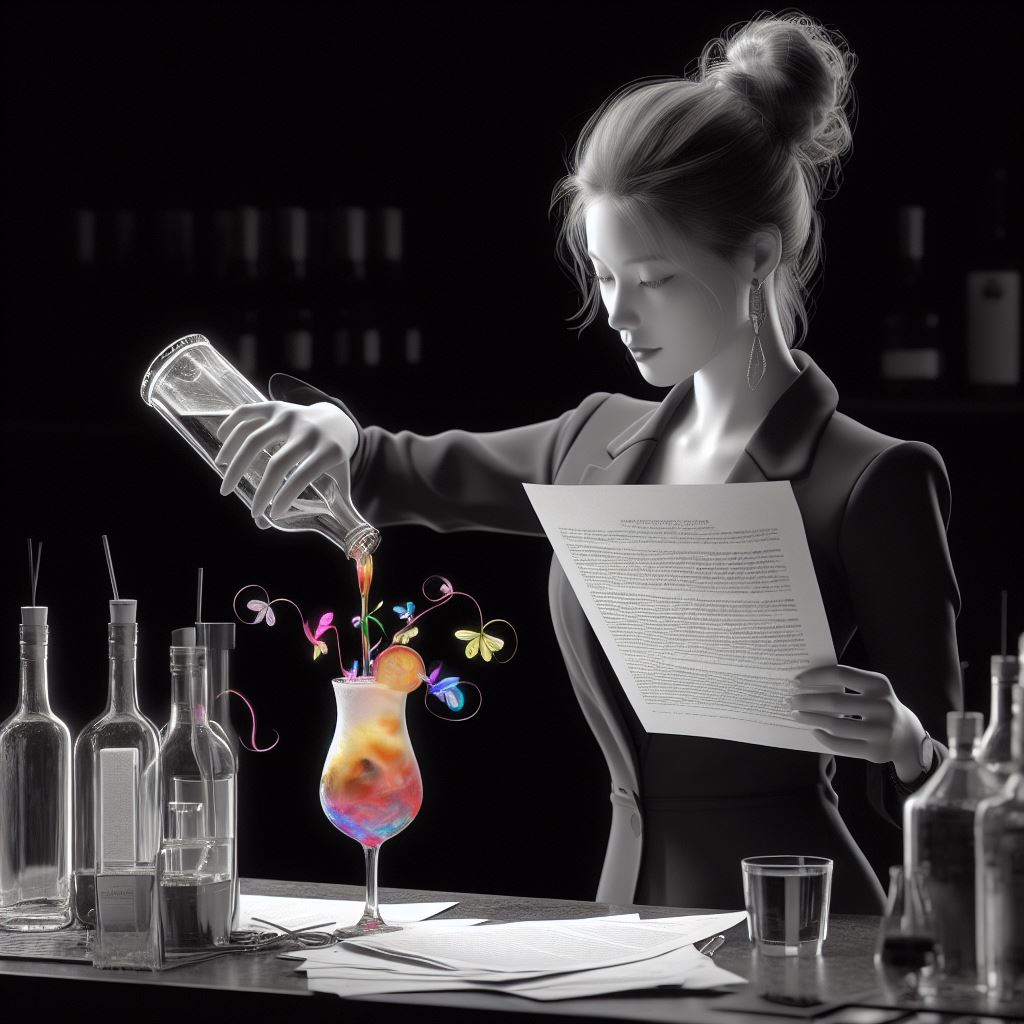
\includegraphics[width=\linewidth]{images/gr_role_1}
            };
        \end{column}
        \begin{column}{0.5\textwidth}
            \begin{tcolorbox}[colback=white,colframe=codegreen,fonttitle=\bfseries, title=Mixmaster Maddy]
                Maddy, a bartender-researcher, considers every paper a cocktail of ideas. She believes in blending theories smoothly. `Stir in a strong conclusion like a punchy cocktail!' she advises while pouring a vibrant concoction. Her reviews are both sharp and intoxicating.
            \end{tcolorbox}
        \end{column}
    \end{columns}
\end{greenframe}

\begin{greenframe}[plain]{Accepting Reviewer}
    \begin{columns}
        \begin{column}{0.5\textwidth}
            \centering
            \tikz\node[inner sep=0pt, draw=none, drop shadow={shadow xshift=1mm,shadow yshift=-1mm,fill=black, opacity=0.3}]{
                
\includegraphics[width=\linewidth]{images/gr_role_2}
            };
        \end{column}
        \begin{column}{0.5\textwidth}
            \begin{tcolorbox}[colback=white,colframe=codegreen,fonttitle=\bfseries, title=Checkout Charlie]
                Berlin's market kingpin, Charlie, is always on the lookout for hidden treasures in papers. `Found some sparkling insights!' he often exclaims. But, just like special offers at checkout, he believes every abstract needs a perk. `How about a dash of humor in the abstract?' he chuckles, scanning items with zest.
            \end{tcolorbox}
        \end{column}
    \end{columns}
\end{greenframe}

\begin{greenframe}[plain]{Accepting Reviewer}
    \begin{columns}
        \begin{column}{0.5\textwidth}
            \centering
            \tikz\node[inner sep=0pt, draw=none, drop shadow={shadow xshift=1mm,shadow yshift=-1mm,fill=black, opacity=0.3}]{
                
\includegraphics[width=\linewidth]{images/gr_role_3}
            };
        \end{column}
        \begin{column}{0.5\textwidth}
            \begin{tcolorbox}[colback=white,colframe=codegreen,fonttitle=\bfseries, title=Kebab King]
                The döner maestro, this man doesn't just wrap kebabs, he wraps praise and critiques together seamlessly. `Such fiery research needs--salate alles und alles drei soße!' he often suggests. Serving sizzling reviews is his forte, often sandwiched with hearty encouragement.
            \end{tcolorbox}
        \end{column}
    \end{columns}
\end{greenframe}

\begin{greenframe}[plain]{Accepting Reviewer}
    \begin{columns}
        \begin{column}{0.5\textwidth}
            \centering
            \tikz\node[inner sep=0pt, draw=none, drop shadow={shadow xshift=1mm,shadow yshift=-1mm,fill=black, opacity=0.3}]{
                
\includegraphics[width=\linewidth]{images/gr_role_4}
            };
        \end{column}
        \begin{column}{0.5\textwidth}
            \begin{tcolorbox}[colback=white,colframe=codegreen,fonttitle=\bfseries, title=Bavarian Brigitte]
                Brigitte, with her classic Bavarian spirit, resonates with Oktoberfest vibes all year round. For her, every commendable paper deserves a hearty `Prost!' With braided hair, traditional dirndl, and infectious enthusiasm, she often says, `Such brilliance! More of this, and the academic world will dance in joy!'
            \end{tcolorbox}
        \end{column}
    \end{columns}
\end{greenframe}

\begin{greenframe}[plain]{Accepting Reviewer}
    \begin{columns}
        \begin{column}{0.5\textwidth}
            \centering
            \tikz\node[inner sep=0pt, draw=none, drop shadow={shadow xshift=1mm,shadow yshift=-1mm,fill=black, opacity=0.3}]{
                
\includegraphics[width=\linewidth]{images/gr_role_5}
            };
        \end{column}
        \begin{column}{0.5\textwidth}
            \begin{tcolorbox}[colback=white,colframe=codegreen,fonttitle=\bfseries, title=Positive Pete]
                Paderborn's pride, Pete's reviews always carry a hint of the historic charm of his hometown. Overflowing with optimism, Pete looks for the silver lining in every research cloud. `Almost there! Just a touch of old-world wisdom will elevate this,' he often remarks, with Paderborn's majestic skyline in his heart.
            \end{tcolorbox}
        \end{column}
    \end{columns}
\end{greenframe}

\begin{greenframe}[plain]{Accepting Reviewer}
    \begin{columns}
        \begin{column}{0.5\textwidth}
            \centering
            \tikz\node[inner sep=0pt, draw=none, drop shadow={shadow xshift=1mm,shadow yshift=-1mm,fill=black, opacity=0.3}]{
                
\includegraphics[width=\linewidth]{images/gr_role_6}
            };
        \end{column}
        \begin{column}{0.5\textwidth}
            \begin{tcolorbox}[colback=white,colframe=codegreen,fonttitle=\bfseries, title=Barbie Bibliophile]
                With her impeccable fashion sense and a love for all things pink, Barbie Bibliophile is here to bring style to the academic world. `Darling, your paper is absolutely fabulous! It's a total runway hit!' she gushes, ever so enchanted by the flair and panache of your writing.
            \end{tcolorbox}
        \end{column}
    \end{columns}
\end{greenframe}

\begin{greenframe}[plain]{Accepting Reviewer}
    \begin{columns}
        \begin{column}{0.5\textwidth}
            \centering
            \tikz\node[inner sep=0pt, draw=none, drop shadow={shadow xshift=1mm,shadow yshift=-1mm,fill=black, opacity=0.3}]{
                
\includegraphics[width=\linewidth]{images/gr_role_7}
            };
        \end{column}
        \begin{column}{0.5\textwidth}
            \begin{tcolorbox}[colback=white,colframe=codegreen,fonttitle=\bfseries, title=Guidance Guru]
                Dwelling under the banyan's shade, this Indian spiritualist reads beyond mere words. `The cosmic energy of your paper resonates with ancient vibrations,' he'd muse. He feels every paper should be rooted in age-old wisdom. `Perhaps blend in some tangible facts to ground this ethereal energy?' is his sage advice.
            \end{tcolorbox}
        \end{column}
    \end{columns}
\end{greenframe}

\begin{greenframe}[plain]{Accepting Reviewer}
    \begin{columns}
        \begin{column}{0.5\textwidth}
            \centering
            \tikz\node[inner sep=0pt, draw=none, drop shadow={shadow xshift=1mm,shadow yshift=-1mm,fill=black, opacity=0.3}]{
                
\includegraphics[width=\linewidth]{images/gr_role_8}
            };
        \end{column}
        \begin{column}{0.5\textwidth}
            \begin{tcolorbox}[colback=white,colframe=codegreen,fonttitle=\bfseries, title=Santa Scholar]
                Santa Scholar is known for his jovial approach to reviewing, always bearing gifts of acceptance. He believes every researcher deserves a bit of holiday cheer. While he sees your mistakes, he’s too focused on the good you've done. `You have been a well-behaved academic! Here's your present: Acceptance!'
            \end{tcolorbox}
        \end{column}
    \end{columns}
\end{greenframe}

\end{document}
